\section{Dataset}
\subsection{Initial Dataset}
\subsection{Enrichments}

\subsection{Statistics}

\paragraph{Motivation}
\label{par:Motivation}
The idea which lays behind these statistics is to get a better understanding of the data we added to the corpus.
In this section, we are going to stress our data, aggregate it, and try to extract some meaning.
We have no pretention to be cinema experts, and there are obvious bias to any statistics which would be built on this data :
\begin{itemize}
    \item First, we are working on a dataset which contains data about less than a thousand movies.
    This is a lot, but at the same time, this is very few, when you know that more than 1450 movies have had an international publication in 2014.
    \item The ratings we base our rankings on are the ratings of ImDB users. Users are not experts.
    Their ratings show how they feel about the movies, but they are not a proof (nor even a direct indicator) that a movie is good or bad.
\end{itemize}

\paragraph{Modus Operandi}
\label{par:ModusOperandi}
All the aggregated statistics you are going to see in this section are based on data aggregated on the condition that there is enough of it.
For instance, in the next section \ref{subs:Director}, we are going to describe which film directors have made the movies that were most (and least) appreciated by the public.
In order to avoid outliers, especially in such a small dataset, we decided not to evaluate the movies from directors of whom only one movie is represented.
This method is not perfect, and to have stronger results, we should have increased this threshold to 5 movies at least.
But the author of our dataset decided not to focus on some specific directors, and to represent as many of them as possible.

\subsubsection{Director}
\label{subs:Director}

\paragraph{Best directors}
\label{par:bestDirectors}


\begin{figure}[!h]
\begin{center}
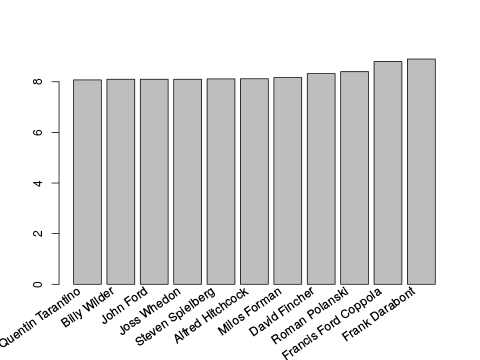
\includegraphics[width=0.70\textwidth]{../src/pre-processing/stats/results/bestDirectors.png}
\end{center}
\caption{Best directors}
\label{fig:bestDirectors}
\end{figure}

\paragraph{Worst directors}
\label{par:worstDirectors}

\begin{figure}[!h]
\begin{center}
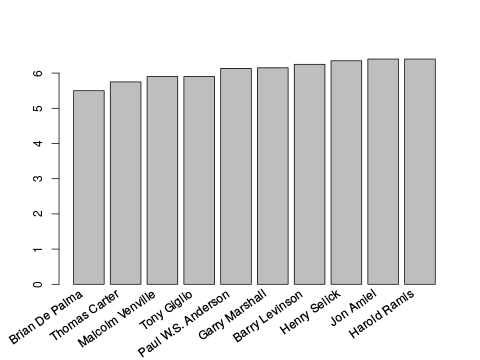
\includegraphics[width=0.70\textwidth]{../src/pre-processing/stats/results/worstDirectors.png}
\end{center}
\caption{Worst directors}
\label{fig:worstDirectors}
\end{figure}

\newpage
\subsubsection{Country}
\label{subs:Country}

\begin{figure}[!h]
\begin{center}
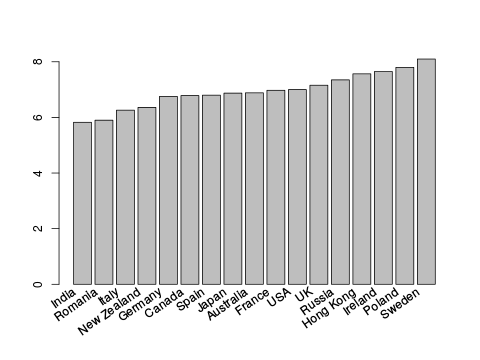
\includegraphics[width=0.70\textwidth]{../src/pre-processing/stats/results/rateByCountry.png}
\end{center}
\caption{Average movie rating for each country}
\label{fig:rateByCountry}
\end{figure}


\newpage
\subsubsection{Ratings}
\label{subs:Ratings}

Is \textit{the old better than the new} ? Not for movies, at least.
Although we would have expected some bias that would play in favour of old movies (Selection \footnote{The movies in this dataset were obviously selected for their diversity, but also for their quality : for an old movie not to be forgotten, it takes more than for a recent one.},
 \textit{Hipstering}, Quantity), it seems that the average rating is getting better with time.
How to interpret that ? Well, an interesting phenomenon is that when you look at the all-time best movies ranking on ImDB, the top movies are either very old, or, most of the time, very recent.
The very old thing can be explained by the combination of two phenomenon :
\begin{itemize}
    \item Quantity : there are more and more movies right now, with bigger and bigger budget.
    So, basically, now, everyone can make his own movie, and try and hide his lack of talent behind massive special effects or famous actors.
    \item Hipstering : for some reason, it is \textit{cool} to like old movies and to promote them as better than the recent blockbusters, which are so \textit{mainstream}.
\end{itemize}
On the other hand, the fact that recent movies are well rated can be explained with a more psychological approach : people tend to like what is new.
Besides, the novelty of a movie like \textit{Avatar} (J.Cameron, 2009) was the mind-blowing special effects, which seem now quite dipappointing, even though the critics were dithyrambic at the time.
For a movie to survive old-fashioned special effects, it takes talent (Confer the fist \textit{Star Wars} trilogy).
That's why recent blockbusters are often disavowed a few years later.

\begin{figure}[!h]
\begin{center}
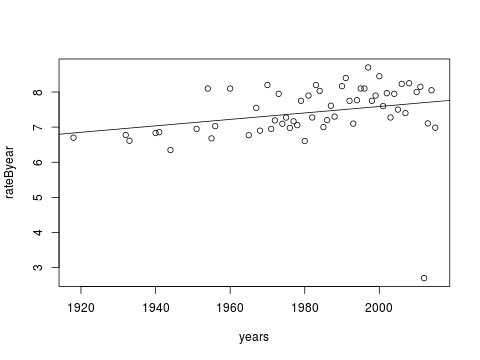
\includegraphics[width=0.70\textwidth]{../src/pre-processing/stats/results/ratingEvolution.png}
\end{center}
\caption{Evolution of rating over time}
\label{fig:ratingEvolution}
\end{figure}

Figure~\ref{fig:ratingPerNbVotes} is also quite interesting.
On the one hand, we could say that there is no direct correlation between the quality of a movie and the quantity of users that evaluated it,
because there are movies evaluated as good with few evaluations, and there are some with many\footnote{Although there are more with few than with many.}.
But on the other hand, movies rated as bad by ImDB users are never evaluated by many users.

\begin{figure}[!h]
\begin{center}
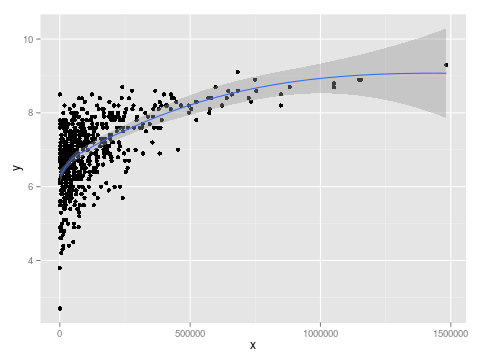
\includegraphics[width=0.70\textwidth]{../src/pre-processing/stats/results/ratingPerNbVotes.png}
\end{center}
\caption{Rating related to amount of ImDB users who voted}
\label{fig:ratingPerNbVotes}
\end{figure}

\newpage
Figure~\ref{fig:ratingPerRuntime} raises the issue of a correlation between rating and runtime.
Well, this is definitely not obvious.
By proceeding a simple least-square linear regression, we can say that the trend is for longer movies to be more appreciated.

\begin{figure}[!h]
\begin{center}
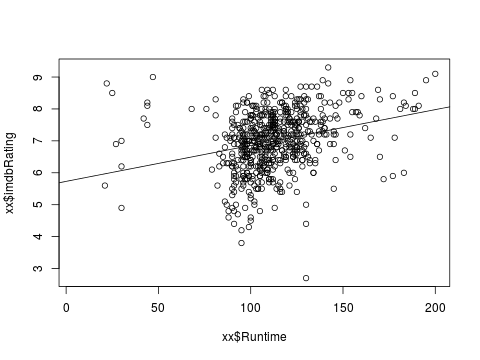
\includegraphics[width=0.70\textwidth]{../src/pre-processing/stats/results/ratingPerRuntime.png}
\end{center}
\caption{Rating related to film duration}
\label{fig:ratingPerRuntime}
\end{figure}

\newpage
\subsubsection{Genre}
\label{subs:Genre}

We can see in Figure~\ref{fig:rateByGenre} that usually, the best ratings are given to movies that deal with serious topics (\textit{History}, \textit{Biography}, \textit{War}).
On the other hand, large-audience topics, such as \textit{Horror} or \textit{Action} movies, or \textit{Comedies}, even though they are very popular, seem to be evaluated as less "good" by the audience.
One surprising result is that \textit{Documentaries} are unexpectedly low in this ranking, when the popular \textit{Drama} is quite high.

\begin{figure}[!h]
\begin{center}
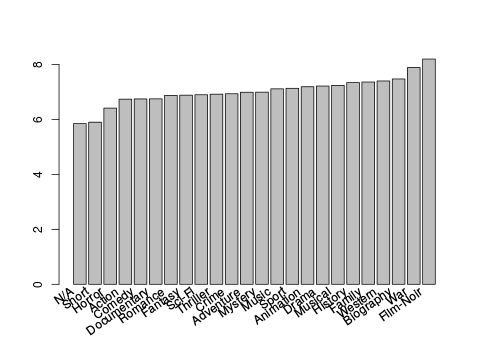
\includegraphics[width=0.70\textwidth]{../src/pre-processing/stats/results/rateByGenre.png}
\end{center}
\caption{Average movie rating for each genre}
\label{fig:rateByGenre}
\end{figure}

In Figure~\ref{fig:dureeByGenre}, we see that the ranking is quite similar as in Figure~\ref{fig:rateByGenre}.
The longer the better : that's a result we already saw in Figure~\ref{fig:ratingPerRuntime} where we evaluated the correlation between rating and duration.
Let's note, though, that most \textit{Films-Noirs} are shorter than the average, and still they get the best ratings.

\begin{figure}[!h]
\begin{center}
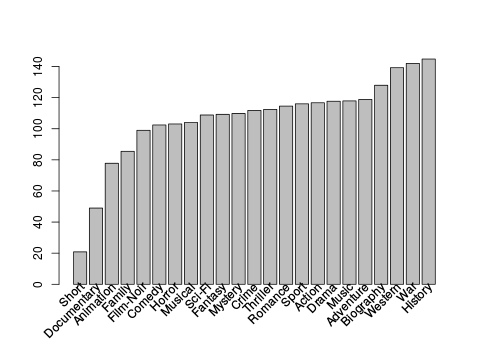
\includegraphics[width=0.70\textwidth]{../src/pre-processing/stats/results/dureeByGenre.png}
\end{center}
\caption{Average movie duration for each genre}
\label{fig:dureeByGenre}
\end{figure}


\newpage
\subsubsection{Actors}
\label{subs:Actors}

\begin{figure}[!h]
\begin{center}
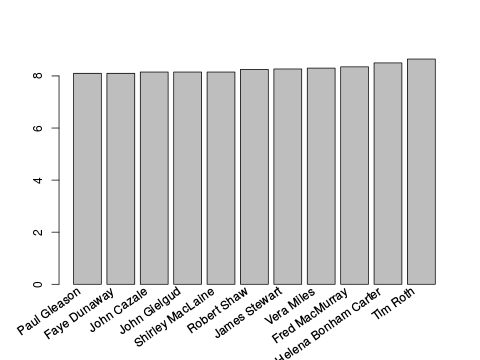
\includegraphics[width=0.70\textwidth]{../src/pre-processing/stats/results/bestActors.png}
\end{center}
\caption{Best actors}
\label{fig:bestActors}
\end{figure}

\begin{figure}[!h]
\begin{center}
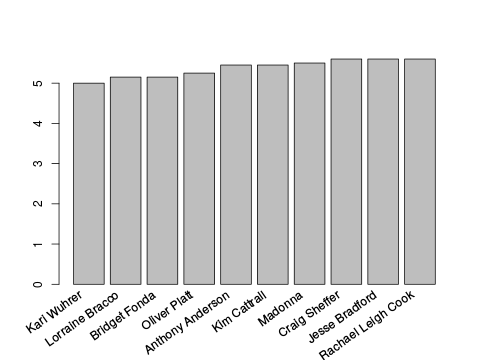
\includegraphics[width=0.70\textwidth]{../src/pre-processing/stats/results/worstActors.png}
\end{center}
\caption{Worst actors}
\label{fig:worstActors}
\end{figure}
